
\documentclass{beamer}
\usepackage{changepage}
\usetheme{default}

\title{Git}

\author{Kiran Vasudev\inst{1}}

\institute[Universities of Somewhere and Elsewhere] 
{
  \inst{1}
  Hochschule Bonn-Rhein-Sieg

}

\begin{document}

\begin{frame}
  \titlepage
\end{frame}

\begin{frame}{Outline}
  \tableofcontents
\end{frame}

\begin{frame}{Introduction}
\section{Introduction}
  \begin{itemize}
  \item {
    Most widely used Version Control System(VCS)
  }
  \item {
    Takes snapshots of the system.
  }
  \end{itemize}
\begin{figure}
	
\includegraphics[scale=0.3]{images/git}
	\caption{Different versions in the form of snapshots\cite{git-basics}}
\end{figure}
\end{frame}

\begin{frame}{Main states of a Git repository}
\section{Main states of a Git repository}
  \begin{itemize}
  \item {
    Working directory
  }
  \item {   
    Staging Area
  }
  \item {   
    .git directory (repository)
  }
  \end{itemize}
	\begin{figure}
		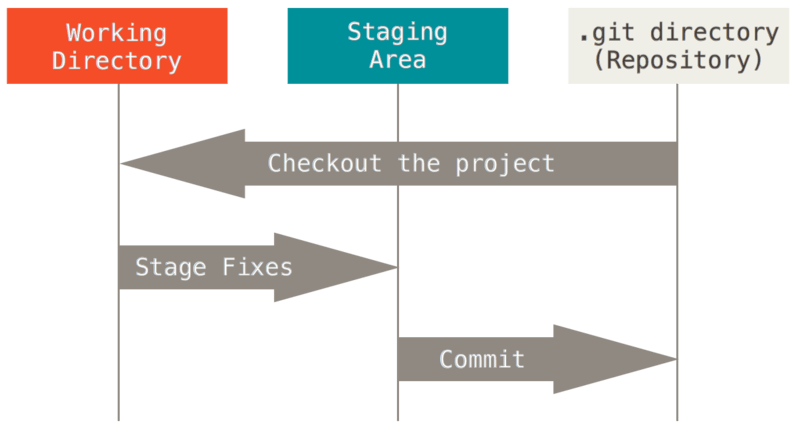
\includegraphics[scale=0.3]{images/areas}
		\caption{Working directory, staging area and the .git directory\cite{git-basics}}
	\end{figure}
\end{frame}

\begin{frame}{States of files in your working directory}
\section{States of files in your working directory}
	\begin{itemize}
		\item Files can either be tracked or untracked.
	\end{itemize}
	\begin{figure}
		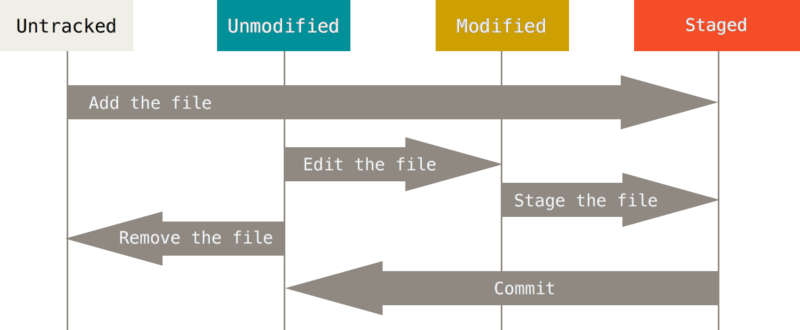
\includegraphics[scale=0.4]{images/lifecycle}
		\caption{Lifecycle of the status of files\cite{recording-changes-git}}
	\end{figure}
\end{frame}	

\begin{frame}[allowframebreaks]{Some important commands}
\section{Some important commands}
\begin{adjustwidth}{-2em}{-2em}
\begin{itemize}
	\item {\textbf{git config --global user.name "user-name"}}
	\item {\textbf{git config --global user.email "email-id"}}
	
	\item {\textbf{git init} \\ Initializes folder to be recognized as a git folder}
	\item {\textbf{git add f\_name }\\ Adds the file to the stage}
	\item {\textbf{git status} \\ To list out the status of files and folders}
	\item {\textbf{git commit -m "message here"} \\ Commits the file to the repository}
	\item {\textbf{git log} \\ Lists the recent commit history}
	
	\item {\textbf{git branch} \\ Lists the available branches}
	\item {\textbf{git checkout b\_name} \\ Switches to another branch}	
\end{itemize}
	
	\begin{itemize}
		\item {\textbf{git clone remote\_location clone\_name} \\ Clones a repository into a new directory}
		\item {\textbf{git remote add remote\_name remote\_location} \\ Remotes are used to track repositories}
		\item {\textbf{git remote -v} \\ Lists all the remotes}
		
		\item {\textbf{git fetch }\\Gathers commits from target branch and stores them in your local repository but does not merge them with the current branch }
		\item {\textbf{git push remote\_name branch\_name}\\Pushes local changes to the remote }
		\item {\textbf{git merge} \\ Merges two development histories together}
		\item {\textbf{git pull}\\Does a git fetch and then a merge}
		
		\item {\textbf{git tag tag\_name} \\ Used to tag a commit}
	\end{itemize}
\end{adjustwidth}
\end{frame}	

\begin{frame}
	\begin{center}
		\Huge Lets get our hands dirty !
	\end{center}
\end{frame}

\begin{frame}{References}
  \section{References}
    
  \begin{thebibliography}{10}

  \bibitem{git-basics}
	\href{https://git-scm.com/book/en/v2/Getting-Started-Git-Basics}{Git basics}
	
  \bibitem{recording-changes-git}
	\href{https://git-scm.com/book/en/v2/Git-Basics-Recording-Changes-to-the-Repository}{Recording changes in Git}
	
	

  \end{thebibliography}
\end{frame}

\end{document}


